\chapter{Release 0 : Mise en place de la plateforme Cloud Native}

\section{Introduction}

La Release 0 constitue le socle technique du projet : trois sprints (Sprint 0, 1, 2) mettent en place les briques d'infrastructure cloud native — cluster Kubernetes, mise à l'échelle serverless via Knative Serving, bus d'événements Kafka opéré par Strimzi — sur lesquelles s'appuient la logique métier et les interfaces des releases suivantes.

Aucune de ces briques n'expose de fonctionnalité à un utilisateur final ; les sprints de cette release ne comportent donc pas de diagramme de cas d'utilisation. Le Chapitre II a présenté l'architecture cible de la plateforme ; ce chapitre documente comment chaque brique a été construite et validée, sprint après sprint.


\section{Sprint 0 : Mise en place de l'infrastructure Kubernetes}

\subsection{Introduction}

Le premier sprint porte sur le socle capable d'accueillir des charges de travail : un cluster Kubernetes à trois nœuds, un plugin réseau (CNI) appliquant l'isolation entre tenants, un mécanisme d'attribution d'adresses IP externes puisque le cluster n'est hébergé chez aucun fournisseur cloud, et une passerelle d'entrée prête pour les applications Knative du sprint suivant. Aucune de ces briques n'est visible pour un utilisateur, mais les choix faits ici, en particulier celui du plugin réseau, se répercutent jusqu'au modèle d'isolation multi-tenant de la plateforme.

\subsection{Objectifs du Sprint}

\begin{itemize}
    \item Mettre en place un cluster Kubernetes à trois nœuds opérationnels, à l'état Ready.
    \item Configurer un réseau de conteneurs (CNI) capable d'appliquer des règles NetworkPolicy entre espaces de noms.
    \item Isoler le trafic réseau entre les futurs tenants de la plateforme.
    \item Attribuer des adresses IP externes aux services LoadBalancer, le cluster n'étant pas hébergé chez un fournisseur cloud.
    \item Mettre en place la passerelle d'entrée Kourier, qui recevra le trafic vers les applications Knative à partir du Sprint 1.
    \item Définir la convention des espaces de noms, un par tenant et un pour la plateforme, ainsi que la convention d'adressage des applications.
\end{itemize}

La plateforme utilise une convention de nommage de la forme <app>.<namespace>.<ip-cluster>.sslip.io. L'adresse IP du cluster est intégrée directement dans le nom d'hôte, et sslip.io la résout automatiquement, sans zone DNS locale à administrer. Ce choix convient à un cluster on-premise en développement, au prix d'une URL moins lisible qu'un domaine dédié.

\subsection{Sprint Backlog}
Le tableau~\ref{tab:sb-sprint0} présente le backlog détaillé du Sprint 0, obtenu en décomposant chaque User Story retenue en tâches techniques.

{
% Le tableau deborde volontairement de 1,5 cm dans chaque marge afin de laisser
% respirer les trois colonnes ; LTleft/LTright sont les parametres propres a
% longtable (adjustwidth n'a aucun effet sur cet environnement).
% Largeur totale : 18,8 cm, soit 1 cm de blanc conserve de chaque cote de la page.
\setlength{\LTleft}{-1.5cm}
\setlength{\LTright}{-1.5cm}
\setlength{\tabcolsep}{8pt}
\renewcommand{\arraystretch}{1.9}
\begin{longtable}{|p{6.6cm}|>{\raggedright\arraybackslash}p{8.1cm}|>{\centering\arraybackslash}p{2.3cm}|}
\hline
User Story & Tâches & Estimation \\
\hline
\endfirsthead
\hline
User Story & Tâches & Estimation \\
\hline
\endhead
\endfoot
\hline
\caption{Backlog du Sprint 0}
\label{tab:sb-sprint0}
\endlastfoot

\multirow{4}{6.6cm}{
\centering
En tant qu'ADMIN, je veux disposer d'un cluster Kubernetes opérationnel afin d'héberger les composants de la plateforme.
}
&
Provisionner le cluster Kubernetes composé d'un control-plane et de deux workers.
& 2 \\*
\cline{2-3}
&
Configurer les nœuds et vérifier leur intégration au cluster.
& 1 \\*
\cline{2-3}
&
Vérifier l'état des trois nœuds et leur disponibilité pour l'exécution des workloads.
& 1 \\*
\cline{2-3}
&
Mettre en place les namespaces nécessaires à l'organisation des workloads et des tenants.
& 1 \\
\hline

\multirow{1}{6.6cm}{
\centering
En tant qu'ADMIN, je veux assurer la connectivité et l'isolation réseau entre les tenants.
}
&
Installer et configurer Cilium comme CNI du cluster Kubernetes.
& 2 \\*
\hline
\cline{2-3}
&
Vérifier le fonctionnement du réseau entre les workloads Kubernetes.
& 1 \\*
\cline{2-3}
&
Définir une politique réseau restrictive de type default-deny pour les namespaces tenants.
& 2 \\*
\cline{2-3}
&
Vérifier l'isolation réseau entre deux namespaces de tenants.
& 2 \\
\hline

\multirow{3}{6.6cm}{
\centering
En tant qu'ADMIN, je veux exposer les services Kubernetes vers le réseau externe.
}
&
Installer et configurer MetalLB dans le cluster on-premise.
& 2 \\*
\cline{2-3}
&
Configurer le mécanisme d'attribution des adresses IP externes aux services de type LoadBalancer.
& 2 \\*
\cline{2-3}
&
Vérifier l'attribution d'une adresse IP externe à un service Kubernetes.
& 1 \\
\hline

\multirow{3}{6.6cm}{
\centering
En tant qu'ADMIN, je veux une passerelle pour les futures applications Knative.
}
&
Installer Kourier comme passerelle d'entrée pour Knative Serving.
& 2 \\*
\cline{2-3}
&
Exposer le service Kourier à l'extérieur du cluster.
& 1 \\*
\cline{2-3}
&
Vérifier l'accessibilité de la passerelle depuis le réseau externe.
& 1 \\
\hline
\end{longtable}
}
% \subsection{Sprint Backlog}

% Le tableau~\ref{tab:sb-sprint0} présente le backlog détaillé du Sprint 0, obtenu en décomposant chaque User Story retenue en tâches techniques.

% % \needspace garantit qu'il reste assez de place sur la page : sans cela une
% % coupure peut tomber au milieu d'un groupe \multirow, dont le contenu deborde
% % alors hors du cadre et laisse une cellule vide sur la page suivante.
% \needspace{0.75\textheight}
% {
% % Le tableau deborde volontairement de 1,5 cm dans chaque marge afin de laisser
% % respirer les trois colonnes ; LTleft/LTright sont les parametres propres a
% % longtable (adjustwidth n'a aucun effet sur cet environnement).
% % Largeur totale : 18,8 cm, soit 1 cm de blanc conserve de chaque cote de la page.
% \setlength{\LTleft}{-1.5cm}
% \setlength{\LTright}{-1.5cm}
% \setlength{\tabcolsep}{8pt}
% \renewcommand{\arraystretch}{1.9}
% \begin{longtable}{|p{6.6cm}|>{\raggedright\arraybackslash}p{8.1cm}|>{\centering\arraybackslash}p{2.3cm}|}
% \hline
% User Story & Tâches & Estimation \\
% \hline
% \endfirsthead
% \hline
% User Story & Tâches & Estimation \\
% \hline
% \endhead
% \endfoot
% \hline

% \caption{Backlog du Sprint 0}
% \label{tab:sb-sprint0}
% \endlastfoot

% \multirow{4}{6.6cm}{
% \centering
% En tant qu'ADMIN, je veux disposer d'un cluster Kubernetes opérationnel afin d'héberger les composants de la plateforme.
% }
% &
% Provisionner le cluster Kubernetes composé d'un control-plane et de deux workers.
% & 2 \\
% \cline{2-3}

% &
% Configurer les nœuds et vérifier leur intégration au cluster.
% & 1 \\
% \cline{2-3}

% &
% Vérifier l'état des trois nœuds et leur disponibilité pour l'exécution des workloads.
% & 1 \\
% \cline{2-3}

% &
% Mettre en place les namespaces nécessaires à l'organisation des workloads et des tenants.
% & 1 \\
% \hline

% \multirow{4}{6.6cm}{
% \centering
% En tant qu'ADMIN, je veux assurer la connectivité et l'isolation réseau entre les tenants.
% }
% &
% Installer et configurer Cilium comme CNI du cluster Kubernetes.
% & 2 \\
% \cline{2-3}

% &
% Vérifier le fonctionnement du réseau entre les workloads Kubernetes.
% & 1 \\
% \cline{2-3}

% &
% Définir une politique réseau restrictive de type default-deny pour les namespaces tenants.
% & 2 \\
% \cline{2-3}

% &
% Vérifier l'isolation réseau entre deux namespaces de tenants.
% & 2 \\
% \hline

% \multirow{3}{6.6cm}{
% \centering
% En tant qu'ADMIN, je veux exposer les services Kubernetes vers le réseau externe.
% }
% &
% Installer et configurer MetalLB dans le cluster on-premise.
% & 2 \\
% \cline{2-3}

% &
% Configurer le mécanisme d'attribution des adresses IP externes aux services de type LoadBalancer.
% & 2 \\
% \cline{2-3}

% &
% Vérifier l'attribution d'une adresse IP externe à un service Kubernetes.
% & 1 \\
% \hline

% \multirow{1}{6.6cm}{
% \centering
% En tant qu'ADMIN, je veux une passerelle pour les futures applications Knative.
% }
% &
% Installer Kourier comme passerelle d'entrée pour Knative Serving.
% & 2 \\
% \hline
% \cline{2-3}

% &
% Exposer le service Kourier à l'extérieur du cluster.
% & 1 \\
% \cline{2-3}

% &
% Vérifier l'accessibilité de la passerelle depuis le réseau externe.
% & 1 \\
% \hline

% \end{longtable}
% }

\subsection{Conception}

\subsubsection{Rôle de Kubernetes et choix d'un cluster on-premise}

Construire une plateforme capable d'exécuter les applications de plusieurs clients sans qu'ils interfèrent entre eux suppose un socle d'orchestration de conteneurs : c'est le rôle de Kubernetes \cite{KubernetesDoc}, qui automatise le placement, le redémarrage et la mise à l'échelle des conteneurs sur un ensemble de machines, en s'appuyant sur le cloisonnement par namespace pour isoler les ressources d'un même cluster.

Ce cloisonnement par namespace est le mécanisme sur lequel repose toute la multi-tenance de la plateforme : chaque client obtient son propre namespace, isolé des autres clients et de la plateforme elle-même. La version exacte de Kubernetes et du container runtime utilisés n'est pas documentée de façon fiable dans le dépôt et n'est donc pas mentionnée ici.

\begin{itemize}
    \item \textbf{Choix d'un cluster on-premise :}\\
    - La plateforme est hébergée sur un cluster bare-metal propre à NextStep IT, plutôt que sur un service Kubernetes managé (EKS, GKE, AKS), cohérent avec les domaines Infrastructure as a Service et Hébergement/Housing de l'intégrateur (cf. Chapitre I), qui dispose ainsi de sa propre infrastructure sans dépendre d'un fournisseur cloud externe. Ce choix justifie directement la nécessité de MetalLB (section~\ref{sec:metallb}), qu'un cluster managé fournirait nativement.
\end{itemize}

\subsubsection{Architecture du cluster de la plateforme}

Le cluster utilisé pour le développement et l'exploitation de la plateforme compte trois nœuds : un nœud de plan de contrôle (control-plane) et deux nœuds de travail (workers). La répartition des rôles et les adresses IP, confirmées par la configuration réseau du backend (notamment sa liste blanche CORS), sont présentées à la figure~\ref{fig:cluster-topology}, qui illustre également la séparation logique entre l'espace de noms de la plateforme et ceux des tenants.

Les caractéristiques matérielles et le système d'exploitation de chaque nœud ne sont pas documentés de façon fiable. Un audit technique réalisé après une première mise en exploitation confirme cette topologie ainsi que la chaîne CNI, LoadBalancer et Ingress décrite dans ce chapitre.

\begin{figure}[H]
\begin{adjustwidth}{-1.0cm}{-1.0cm}
\centering
\begin{tikzpicture}[
  x=1cm, y=1cm,
  every node/.style={font=\normalsize},
  vm/.style={draw=figVert, line width=1pt, rounded corners, minimum width=4.2cm,
             minimum height=1.6cm, align=center, fill=figVertFond},
  cp/.style={draw=figVert, line width=1.4pt, rounded corners, minimum width=4.2cm,
             minimum height=1.6cm, align=center, fill=figVertFond!60!white},
  nsp/.style={draw=figBleu, line width=1pt, rounded corners, minimum width=6.4cm,
              minimum height=2.7cm, align=center, fill=figBleuFond},
  nst/.style={draw=figOrange, line width=1pt, dashed, rounded corners, minimum width=6.4cm,
              minimum height=2.7cm, align=center, fill=figOrangeFond},
  couche/.style={draw=black!40, dotted, line width=0.9pt, rounded corners, inner sep=12pt},
  ttl/.style={font=\small\bfseries, text=black!65}
]

% ---- couche physique : le plan de controle au centre, une liaison droite vers chaque worker ----
\node[vm] (vm02) at (0,0)    {vm02\\[1pt]\small worker\\\small 10.9.21.224};
\node[cp] (vm01) at (6.2,0)  {vm01\\[1pt]\small plan de contrôle\\\small 10.9.21.223};
\node[vm] (vm03) at (12.4,0) {vm03\\[1pt]\small worker\\\small 10.9.21.225};

\draw[<->, line width=1pt, figVert] (vm02) -- (vm01)
      node[midway, above=0pt, font=\scriptsize, fill=white, inner sep=1.5pt] {API Kubernetes};
\draw[<->, line width=1pt, figVert] (vm01) -- (vm03)
      node[midway, above=0pt, font=\scriptsize, fill=white, inner sep=1.5pt] {API Kubernetes};

\node[couche, fit=(vm02)(vm01)(vm03)] (phys) {};
\node[ttl, anchor=south west] at ([yshift=3pt]phys.north west) {Couche physique : trois nœuds};

% ---- couche logique : partition en namespaces ----
\node[nsp] (plat) at (2.6,-6.2)
     {Namespace \texttt{platform}\\[4pt]
      \small backend-api \quad web-portal\\\small admin-console\\\small PostgreSQL \quad Keycloak};
\node[nst] (ten) at (10.6,-6.2)
     {Namespace \texttt{user-<tenant>}\\[4pt]
      \small applications du client\\\small NetworkPolicy default-deny\\[2pt]
      \footnotesize\itshape un namespace par client, créé à la volée};

\node[couche, fit=(plat)(ten)] (logi) {};
\node[ttl, anchor=south west] at ([yshift=3pt]logi.north west) {Couche logique : namespaces};

% ---- articulation entre les deux couches ----
\draw[->, line width=1pt, black!55] (6.2,-1.9) -- (6.2,-3.6);
\node[font=\scriptsize, text=black!70, align=left, anchor=west] at (6.6,-2.75)
     {les Pods d'un namespace s'exécutent indifféremment\\sur \texttt{vm02} ou \texttt{vm03} : la répartition est logique,\\pas physique};

\end{tikzpicture}
\caption{Architecture du cluster Kubernetes de la plateforme}
\label{fig:cluster-topology}
\end{adjustwidth}
\end{figure}

Le namespace \texttt{user-<tenant>}, créé dynamiquement pour chaque client, contient ses applications déployées ainsi qu'une règle d'isolation réseau, détaillée ci-après.

\subsubsection{Isolation réseau des tenants : le CNI et Cilium}

Isoler des namespaces sur le papier ne suffit pas : il faut que le réseau du cluster respecte réellement cette séparation. Kubernetes délègue cette responsabilité à un plugin CNI (Container Network Interface), chargé d'attribuer une adresse IP à chaque Pod et d'acheminer le trafic.

Le CNI retenu est Cilium \cite{CiliumDoc}, choisi pour sa prise en charge des NetworkPolicy et son architecture eBPF, plus performante que les règles iptables traditionnelles et ouverte vers de l'observabilité réseau avancée. Comparé à Flannel, qui ne supporte pas nativement les NetworkPolicy, et à Calico, qui les supporte de façon comparable, Cilium a été retenu pour ce potentiel d'évolution. Un audit technique de la plateforme confirme ce choix comme robuste.

\paragraph{La NetworkPolicy réelle du projet.}\mbox{}\par
Une politique réseau de type default-deny (\texttt{k8s/tenant/network-policy.yaml}) est créée automatiquement pour chaque nouveau namespace tenant par le backend applicatif, un mécanisme détaillé au chapitre consacré à son développement (Release 1). Elle bloque par défaut tout trafic non explicitement autorisé entre Pods, et n'ouvre sélectivement que les flux nécessaires au fonctionnement de la plateforme : composants système (Kourier, Knative Serving, monitoring), résolution DNS, et bus d'événements Kafka partagé. Le trafic direct entre deux tenants reste refusé par défaut, garantissant qu'un client ne peut pas atteindre les ressources d'un autre, même en connaissant son adresse interne. La figure~\ref{fig:cilium-isolation} illustre ce principe.

\begin{figure}[H]
 \centering
    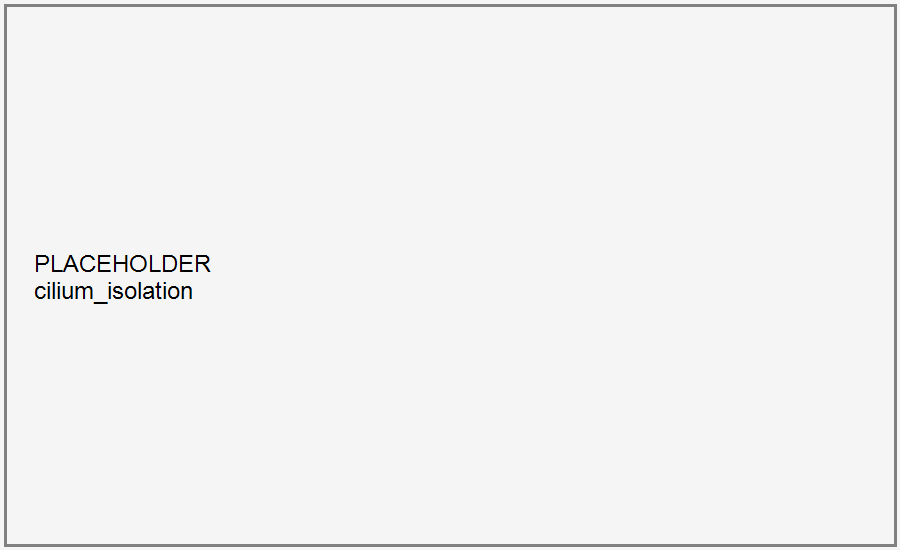
\includegraphics[width=0.85\textwidth]{image/cilium_isolation.png}
    \caption{Isolation réseau entre tenants via Cilium}
    \label{fig:cilium-isolation}
\end{figure}

\subsubsection{Exposition externe des services : MetalLB}
\label{sec:metallb}

Sur un cluster hébergé chez un fournisseur cloud public, un service LoadBalancer reçoit automatiquement une adresse IP publique — un mécanisme absent d'un cluster on-premise, où un tel service resterait indéfiniment à l'état \texttt{pending}. MetalLB \cite{MetalLBDoc} comble ce manque en attribuant, depuis l'intérieur du cluster, des adresses IP externes puisées dans une plage réservée du réseau local.

Sur la plateforme, le portail client \texttt{platform-web} est exposé directement en LoadBalancer et obtient l'adresse 10.9.21.238. La console d'administration \texttt{platform-admin} reste volontairement en NodePort fixe (port 30081), cohérent avec son accès aux fonctions d'administration globale. Le manifeste MetalLB n'est pas versionné dans le dépôt ; seule son utilisation effective est confirmée. La figure~\ref{fig:metallb-flux} illustre ce flux d'attribution.

\begin{figure}[H]
\begin{adjustwidth}{-1.0cm}{-1.0cm}
\centering
\begin{tikzpicture}[
  x=1cm, y=1cm,
  every node/.style={font=\normalsize},
  k8s/.style={draw=figVert, line width=1pt, rounded corners, minimum width=6.4cm,
              minimum height=1.4cm, align=center, fill=figVertFond},
  res/.style={draw=figOrange, line width=1pt, rounded corners, minimum width=6.0cm,
              minimum height=1.15cm, align=center, fill=figOrangeFond, font=\small},
  cli/.style={draw=figBleu, line width=1pt, rounded corners, minimum width=6.4cm,
              minimum height=1.4cm, align=center, fill=figBleuFond},
  note/.style={draw=black!45, dashed, line width=0.9pt, rounded corners, align=left,
               font=\small, fill=black!3},
  cadre/.style={draw=figOrange, dashed, line width=1.1pt, rounded corners, inner sep=11pt},
  num/.style={circle, draw, line width=0.8pt, fill=white, inner sep=2pt, font=\small\bfseries},
  lbl/.style={font=\small},
  fl/.style={->, line width=1pt, figVert}
]

\node[k8s] (svc) at (0,0)
     {Service \texttt{platform-web}\\[1pt]\small \texttt{type: LoadBalancer}};

% Sans MetalLB : l'etat terminal sur un cluster on-premise.
\node[note] (pend) at (8.6,0)
     {Sur un cluster on-premise, sans MetalLB\\
      \texttt{EXTERNAL-IP} reste \texttt{<pending>}\\
      indéfiniment : aucun contrôleur n'attribue d'IP};
\draw[->, line width=1pt, black!45, dashed] (svc.east) -- (pend.west);

% Le composant MetalLB et ses deux ressources.
\node[res] (ctrl) at (0,-3.2) {controller : observe les Services \texttt{LoadBalancer}};
\node[res] (pool) at (0,-4.7) {IPAddressPool : plage réservée du réseau local};
\node[cadre, fit=(ctrl)(pool)] (mlb) {};
\node[font=\small\bfseries, text=figOrange, anchor=south west]
      at ([yshift=3pt]mlb.north west) {MetalLB};

\node[k8s] (ip) at (0,-7.5)
     {\texttt{EXTERNAL-IP} : 10.9.21.238\\[1pt]\small l'adresse devient joignable sur le réseau local};

\node[cli] (client) at (0,-10.1)
     {Client externe\\[1pt]\small atteint le portail sur \texttt{10.9.21.238}};

\draw[fl] (svc.south) -- (mlb.north);
\draw[fl] (mlb.south) -- (ip.north);
\draw[->, line width=1pt, figBleu] (ip.south) -- (client.north);

\node[num] at (0,-1.47) {1};
\node[num] at (0,-6.23) {2};
\node[num] at (0,-8.80) {3};

\node[lbl, anchor=west] at (0.35,-1.47) {le Service demande une IP externe};
\node[lbl, anchor=west] at (0.35,-6.23) {MetalLB attribue puis annonce l'adresse};
\node[lbl, anchor=west] at (0.35,-8.80) {le trafic entre dans le cluster};

% Le cas volontairement different de la console d'administration.
\node[note, text=black!80] at (9.0,-8.80)
     {Cas de \texttt{platform-admin}\\
      non exposée par MetalLB : accès en\\
      \texttt{NodePort} fixe sur le port 30081,\\
      restriction volontaire liée à ses\\
      fonctions d'administration globale};

\end{tikzpicture}
\caption{Attribution d'une adresse IP externe via MetalLB}
\label{fig:metallb-flux}
\end{adjustwidth}
\end{figure}

\subsubsection{Passerelle d'entrée pour Knative : Kourier}

Une fois l'IP externe attribuée, Kourier \cite{KourierDoc} achemine chaque requête vers la bonne application : il reçoit le trafic HTTP destiné aux services Knative Serving et le route vers la Revision active selon le nom d'hôte, conforme à la convention présentée en introduction de ce sprint. Son installation, indissociable du fonctionnement de Knative Serving, est présentée au Sprint 1.

La figure~\ref{fig:architecture-reseau} synthétise la chaîne complète mise en place par ce sprint, pour une requête HTTP externe à destination d'une application tenant.

\begin{figure}[H]
\centering
\begin{tikzpicture}[node distance=1cm, every node/.style={font=\small}]
\tikzstyle{box}=[draw, rounded corners, minimum width=2.3cm, minimum height=0.9cm, align=center, fill=Gray!20]
\node[box] (client) {Client externe};
\node[box, right=1cm of client] (metallb) {MetalLB\\(IP externe)};
\node[box, right=1cm of metallb] (kourier) {Kourier\\(ingress gateway)};
\node[box, right=1cm of kourier] (svc) {Service\\namespace tenant};
\draw[->, thick] (client) -- (metallb);
\draw[->, thick] (metallb) -- (kourier);
\draw[->, thick] (kourier) -- (svc);
\end{tikzpicture}
\caption{Chemin d'une requête externe vers une application tenant}
\label{fig:architecture-reseau}
\end{figure}

\subsection{Réalisation}

\subsubsection{Mise en œuvre}

Ce sprint livre quatre composants, tous opérationnels à la date de rédaction : le cluster Kubernetes à trois nœuds, Cilium pour le réseau des Pods et les NetworkPolicy, MetalLB pour l'attribution d'IP externes, et Kourier comme passerelle d'entrée pour Knative Serving. La convention d'espaces de noms distingue le namespace \texttt{platform}, qui héberge les composants de la plateforme, des namespaces créés dynamiquement, un par tenant, lors du premier déploiement — une création prise en charge par le backend et détaillée au chapitre qui lui est consacré (Release 1).

\begin{itemize}
    \item \textbf{État des nœuds du cluster:}
\end{itemize}

La figure~\ref{fig:capture-nodes} confirme l'état Ready des trois nœuds, avec les versions observées : Kubernetes v1.30.3, Ubuntu 24.04.4 LTS, containerd 2.2.1.

\begin{figure}[H]
\centering
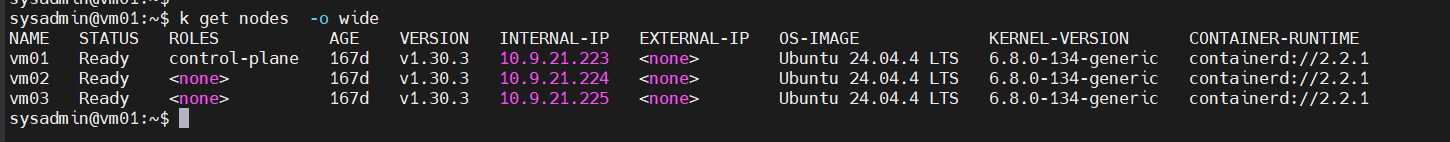
\includegraphics[width=0.9\textwidth]{image/capture_kubectl_get_nodes.png}
\caption{État des nœuds du cluster: }
\label{fig:capture-nodes}
\end{figure}

\begin{itemize}
    \item \textbf{État de Cilium:}
\end{itemize}

La figure~\ref{fig:capture-cilium-status} confirme l'état OK de Cilium, Envoy et l'opérateur, en version 1.19.1.

\begin{figure}[H]
\centering
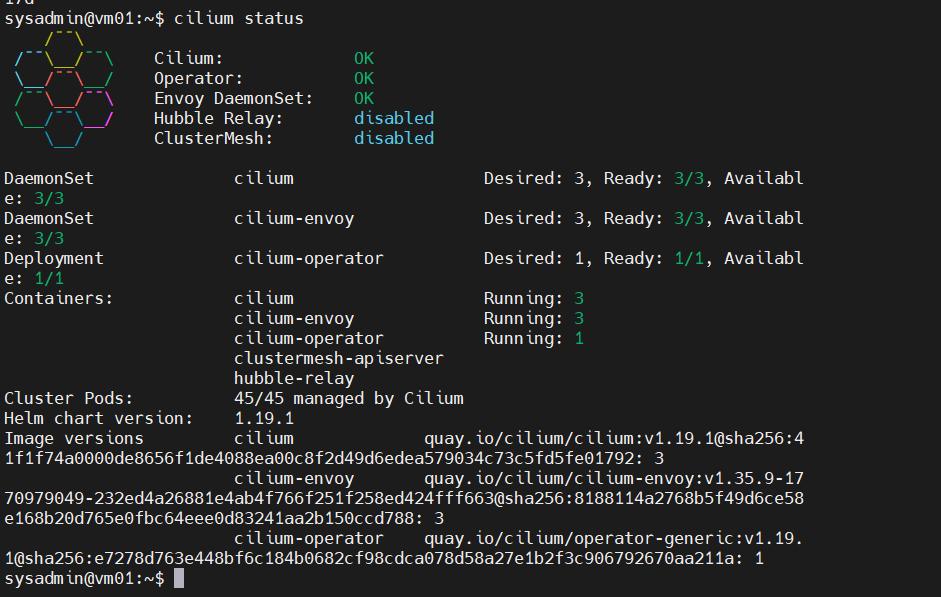
\includegraphics[width=0.85\textwidth]{image/capture_cilium_status.png}
\caption{État de Cilium}
\label{fig:capture-cilium-status}
\end{figure}

\begin{itemize}
    \item \textbf{Pods d'infrastructure réseau:}
\end{itemize}

La figure~\ref{fig:capture-pods-infra} montre les pods \texttt{kube-system} et \texttt{metallb-system} à l'état Running. On y observe une duplication non expliquée de Kourier, présent à la fois sous \texttt{net-kourier-controller} et sous une passerelle \texttt{3scale-kourier-gateway}, dans deux namespaces distincts.

\begin{figure}[H]
\centering
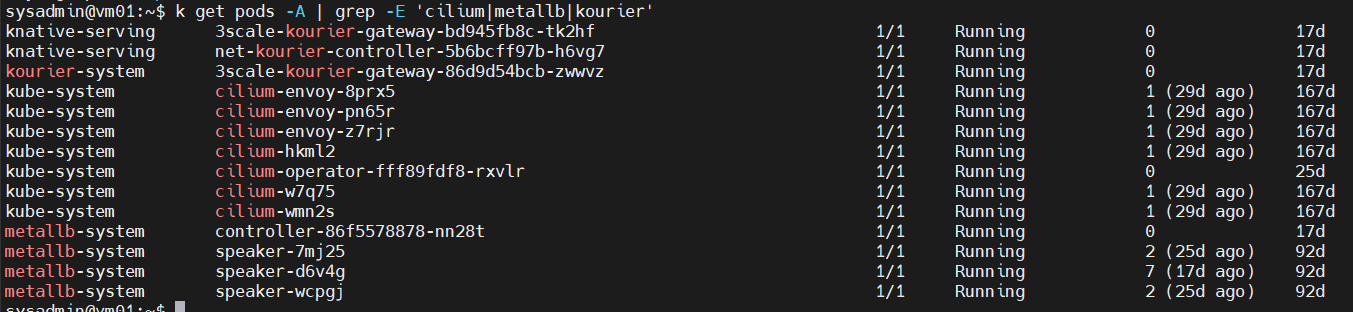
\includegraphics[width=0.9\textwidth]{image/capture_pods_infra.png}
\caption{Pods d'infrastructure réseau}
\label{fig:capture-pods-infra}
\end{figure}

\begin{itemize}
    \item \textbf{Namespaces du cluster:}
\end{itemize}

La figure~\ref{fig:capture-ns} confirme la présence du namespace \texttt{platform} et de quatre namespaces tenants.

\begin{figure}[H]
\centering
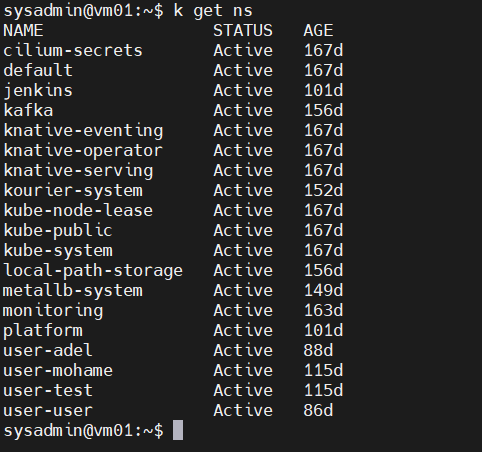
\includegraphics[width=0.85\textwidth]{image/capture_get_namespaces.png}
\caption{Namespaces du cluster}
\label{fig:capture-ns}
\end{figure}

\begin{itemize}
    \item \textbf{Politiques réseau des tenants:}
\end{itemize}

La figure~\ref{fig:capture-netpol} révèle un écart réel : seul le namespace \texttt{user-user} possède la règle \texttt{tenant-default-isolation}. Les trois autres n'en ont aucune, un point non expliqué dans le dépôt et retenu comme limite de ce sprint.

\begin{figure}[H]
\centering
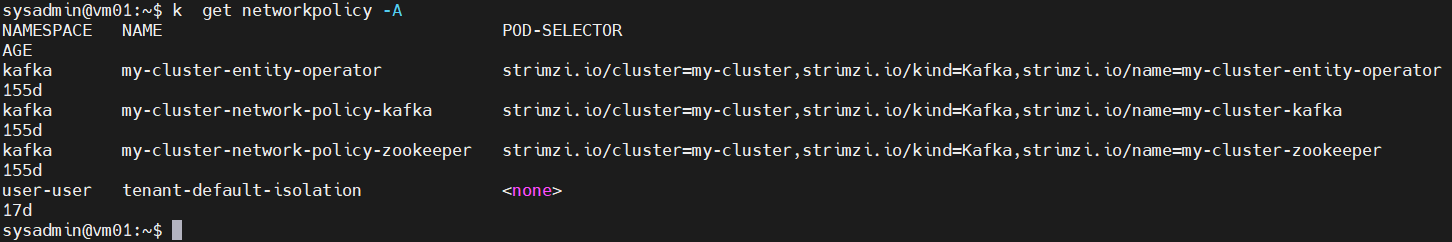
\includegraphics[width=0.85\textwidth]{image/capture_get_networkpolicy.png}
\caption{Politiques réseau des tenants}
\label{fig:capture-netpol}
\end{figure}

\section{Sprint 1 : Déploiement de Knative Serving}

\subsection{Introduction}

Le cluster livré au sprint précédent héberge des conteneurs, mais rien n'y automatise encore leur mise à l'échelle selon le trafic reçu. Knative Serving comble ce manque : son installation, son raccordement à la passerelle Kourier déjà en place et sa pilotabilité depuis le backend constituent le cœur de ce sprint. Un point conditionne toute l'intégration : il n'existe pas de client Java officiel pour les ressources Knative, ce qui impose de passer par l'API générique de Fabric8, avec les limites discutées plus loin dans ce sprint.

\subsection{Objectifs du Sprint}

\begin{itemize}
    \item Installer Knative Serving et l'intégrer à la passerelle Kourier mise en place au Sprint 0.
    \item Permettre au backend de créer une ressource Service Knative par programmation, via Fabric8.
    \item Créer automatiquement le namespace d'un tenant et sa NetworkPolicy lors de son premier déploiement.
\end{itemize}

\subsection{Sprint Backlog}

Le tableau~\ref{tab:sb-sprint1} présente le backlog détaillé du Sprint 1, obtenu en décomposant chaque User Story retenue en tâches techniques.

% \needspace garantit qu'il reste assez de place sur la page : sans cela une
% coupure peut tomber au milieu d'un groupe \multirow, dont le contenu deborde
% alors hors du cadre et laisse une cellule vide sur la page suivante.
\needspace{0.75\textheight}
{
% Le tableau deborde volontairement de 1,5 cm dans chaque marge afin de laisser
% respirer les trois colonnes ; LTleft/LTright sont les parametres propres a
% longtable (adjustwidth n'a aucun effet sur cet environnement).
% Largeur totale : 18,8 cm, soit 1 cm de blanc conserve de chaque cote de la page.
\setlength{\LTleft}{-1.5cm}
\setlength{\LTright}{-1.5cm}
\setlength{\tabcolsep}{8pt}
\renewcommand{\arraystretch}{1.9}
\begin{longtable}{|p{6.6cm}|>{\raggedright\arraybackslash}p{8.1cm}|>{\centering\arraybackslash}p{2.3cm}|}
\hline
User Story & Tâches & Estimation \\
\hline
\endfirsthead
\hline
User Story & Tâches & Estimation \\
\hline
\endhead
\endfoot
\hline

\caption{Backlog du Sprint 1}
\label{tab:sb-sprint1}
\endlastfoot

\multirow{2}{6.6cm}{
\centering
En tant qu'ADMIN, je veux que Knative Serving soit opérationnel sur le cluster.
}
&
Installer Knative Serving et l'intégrer à la passerelle Kourier mise en place au Sprint 0.
& 3 \\
\cline{2-3}

&
Vérifier qu'un Service Knative de test atteint la condition Ready et expose une URL.
& 1 \\
\hline

\multirow{3}{6.6cm}{
\centering
En tant que développeur backend, je veux pouvoir créer une ressource Knative Service par programmation.
}
&
Implémenter la création d'une ressource Service Knative via l'API générique Fabric8.
& 3 \\
\cline{2-3}

&
Vérifier que le service créé est visible via kubectl get ksvc, avec l'image demandée.
& 1 \\
\cline{2-3}

&
Observer le cycle Service vers Revision et le comportement d'autoscaling.
& 2 \\
\hline

\multirow{3}{6.6cm}{
\centering
En tant que système, je veux que l'espace de noms d'un tenant soit créé automatiquement au premier déploiement.
}
&
Implémenter la création automatique du namespace tenant et de sa NetworkPolicy au premier déploiement.
& 2 \\
\cline{2-3}

&
Vérifier l'existence du namespace et de la NetworkPolicy après un premier déploiement.
& 1 \\
\cline{2-3}

&
Observer le comportement de scale-to-zero natif de Knative.
& 2 \\
\hline

\end{longtable}
}

\subsection{Conception}

\subsubsection{Knative Serving : rôle et concepts}

Le cluster du Sprint 0 exécute des Pods et isole les tenants, mais ne gère pas encore leur nombre selon la charge. Knative Serving \cite{KnativeServingDoc} ajoute cette capacité : il fait tourner une application uniquement quand elle reçoit du trafic, et coupe les instances inutilisées.

Trois ressources le structurent : le Service (image, port, ressources, bornes de mise à l'échelle), la Revision (instantané figé de la configuration, créé à chaque modification du Service) et la Route (distribue le trafic vers une ou plusieurs révisions).

Knative ajuste le nombre de Pods d'une révision selon le trafic et peut le réduire jusqu'à zéro instance en l'absence de sollicitation (le scale-to-zero, illustré figure~\ref{fig:scale-to-zero}), avant qu'une nouvelle requête ne réactive automatiquement une instance.

\begin{figure}[H]
\begin{adjustwidth}{-1.3cm}{-1.3cm}
\centering
\begin{tikzpicture}[
  x=1cm, y=1cm,
  every node/.style={font=\normalsize},
  don/.style={draw=figBleu, line width=1pt, rounded corners, minimum width=6.0cm,
              minimum height=1.45cm, align=center, fill=figBleuFond},
  eta/.style={draw=figVert, line width=1pt, rounded corners, minimum width=6.0cm,
              minimum height=1.45cm, align=center, fill=figVertFond},
  ctl/.style={draw=figOrange, line width=1pt, dashed, rounded corners, minimum width=5.0cm,
              minimum height=1.45cm, align=center, fill=figOrangeFond},
  num/.style={circle, draw, line width=0.8pt, fill=white, inner sep=2pt, font=\small\bfseries},
  lbl/.style={font=\small},
  fl/.style={->, line width=1pt, figBleu},
  fv/.style={->, line width=1pt, figVert},
  fc/.style={->, line width=1pt, dashed, figOrange}
]

\node[eta] (s0)  at (0,0)     {État de repos : 0 Pod\\[1pt]\small la Route pointe vers l'Activator};
\node[don] (kou) at (0,-2.6)  {Kourier\\[1pt]\small passerelle d'entrée du cluster};
\node[don] (act) at (0,-5.2)  {Activator\\[1pt]\small met la requête en file d'attente};
\node[don] (pod) at (0,-9.4)  {Pod : \texttt{queue-proxy} + conteneur\\[1pt]\small l'application traite la requête};
\node[eta] (fin) at (0,-12.2) {Retour au repos\\[1pt]\small les Pods sont supprimés};

\node[ctl] (kpa)  at (9.4,-5.2)  {Autoscaler (KPA)};
\node[ctl] (rev)  at (9.4,-7.3)  {Revision $\rightarrow$ Deployment\\[1pt]\small réplicas 0 $\rightarrow$ 1};
\node[ctl] (down) at (9.4,-12.2) {Autoscaler\\[1pt]\small réplicas 1 $\rightarrow$ 0};

\draw[fl] (s0)  -- (kou);
\draw[fl] (kou) -- (act);
\draw[fc] (act.east) -- (kpa.west);
\draw[fc] (kpa) -- (rev);
\draw[fl] (rev.south) |- ([yshift=0.35cm]pod.east);
\draw[fl] (act) -- (pod);
\draw[fc] ([yshift=-0.35cm]pod.east) -- (13.0,-9.75) |- (kpa.east);
\draw[fv] (pod) -- (fin);
\draw[fc] (fin.east) -- (down.west);
\draw[fv] (down.east) -- (14.4,-12.2) |- (s0.east);

\node[lbl, anchor=east]  at (-0.3,-1.3)  {requête HTTP};
\node[lbl, anchor=south] at (4.7,-5.0)   {signale la demande};
\node[lbl, anchor=south] at (6.0,-9.3)   {le Pod démarre};
\node[lbl, anchor=east]  at (-0.3,-7.3)  {transmet la requête};
\node[lbl, anchor=north] at (7.6,-9.95)  {métriques de concurrence};
\node[lbl, anchor=east]  at (-0.3,-10.8) {inactivité prolongée};
\node[lbl, anchor=south] at (8.5,0.2)    {nouveau cycle};

\node[num] at (0,-1.3)    {1};
\node[num] at (0,-3.9)    {2};
\node[num] at (4.7,-5.2)  {3};
\node[num] at (9.4,-6.25) {4};
\node[num] at (6.0,-9.05) {5};
\node[num] at (0,-7.3)    {6};
\node[num] at (13.0,-7.5) {7};
\node[num] at (0,-10.8)   {8};
\node[num] at (4.7,-12.2) {9};

\end{tikzpicture}
\caption{Cycle complet de mise à zéro et de réveil automatique d'un service Knative}
\label{fig:scale-to-zero}
\end{adjustwidth}
\end{figure}

Ce comportement est natif à Knative et n'est pas réimplémenté par le backend. Sa preuve concrète nécessite une séquence d'observation dans le temps, non disponible à la date de rédaction.

% TODO: figures réelles à ajouter — trois captures de kubectl get pods
% -n <namespace-tenant> : (1) 1 Pod actif, (2) 0 Pod après inactivité,
% (3) 1 Pod après une nouvelle requête (preuve du scale-to-zero, S1-V05).

\subsubsection{Intégration avec Kubernetes et le backend}

Une ressource Service Knative n'est pas un objet Kubernetes natif : c'est une CRD (Custom Resource Definition), au même titre que les ressources ajoutées par Strimzi pour Kafka au Sprint 2. Elle suit le même modèle de namespace, ce qui la fait bénéficier de la NetworkPolicy default-deny du tenant concerné.

Le backend pilote cette ressource (création, lecture de statut, gestion des révisions) via la bibliothèque Fabric8 Kubernetes Client~\cite{Fabric8Doc} ; son implémentation précise est présentée au chapitre consacré au backend (Release 1). La figure~\ref{fig:backend-knative-integration} situe cette intégration dans la chaîne complète, du backend jusqu'au Pod applicatif.

\begin{figure}[H]
\begin{adjustwidth}{-1.3cm}{-1.3cm}
\centering
\begin{tikzpicture}[
  x=1cm, y=1cm,
  every node/.style={font=\normalsize},
  bk/.style={draw=figBleu, line width=1pt, rounded corners, minimum width=5.6cm,
             minimum height=1.45cm, align=center, fill=figBleuFond},
  k8s/.style={draw=figVert, line width=1pt, rounded corners, minimum width=5.6cm,
              minimum height=1.45cm, align=center, fill=figVertFond},
  crd/.style={draw=figOrange, line width=1pt, dashed, rounded corners, minimum width=5.6cm,
              minimum height=1.45cm, align=center, fill=figOrangeFond},
  lbl/.style={font=\small},
  fl/.style={->, line width=1pt, figBleu},
  fo/.style={->, line width=1pt, figOrange}
]

\node[bk]  (back) at (0,0)    {Backend Spring Boot\\[1pt]\small paramètres saisis par le client};
\node[bk]  (fab)  at (0,-2.6) {Fabric8 Kubernetes Client\\[1pt]\small construit le manifeste};
\node[k8s] (api)  at (0,-5.2) {API Kubernetes\\[1pt]\small \texttt{kube-apiserver}};

\node[crd] (svc)  at (8.8,-5.2)  {Service Knative (CRD)\\[1pt]\small dans le namespace du tenant};
\node[crd] (rev)  at (8.8,-7.8)  {Revision\\[1pt]\small instantané figé de la configuration};
\node[crd] (dep)  at (8.8,-10.4) {Deployment\\[1pt]\small géré par Knative Serving};
\node[k8s] (pod)  at (8.8,-13.0) {Pod applicatif\\[1pt]\small \texttt{queue-proxy} + conteneur client};

\draw[fl] (back) -- (fab);
\draw[fl] (fab)  -- (api);
\draw[fl] (api)  -- (svc);
\draw[fo] (svc)  -- (rev);
\draw[fo] (rev)  -- (dep);
\draw[fo] (dep)  -- (pod);

\node[lbl, anchor=east, align=right] at (-0.3,-1.3) {image, port, ressources,\\bornes de mise à l'échelle};
\node[lbl, anchor=east, align=right] at (-0.3,-3.9) {soumet la ressource\\personnalisée};
\node[lbl, anchor=south] at (4.4,-5.0)  {crée la CRD};

\node[draw=figVert, line width=1pt, rounded corners, fill=figVertFond, align=left,
      font=\small, minimum width=6.0cm] (notes) at (1.0,-13.0)
      {Hérité du namespace du tenant\\[2pt]
       $\bullet$ NetworkPolicy default-deny (Sprint 0)\\
       $\bullet$ variables d'environnement Kafka\\
       \quad injectées automatiquement (Strimzi)};
\draw[->, line width=1pt, dashed, figVert] (notes.east) -- (pod.west);

\end{tikzpicture}
\caption{Chaîne d'intégration du backend à Knative Serving}
\label{fig:backend-knative-integration}
\end{adjustwidth}
\end{figure}

Le manifeste soumis reprend les paramètres fournis par le client : image et tag Docker, port d'écoute (8080 par défaut), ressources demandées (100m CPU / 128Mi mémoire par défaut), et bornes minScale/maxScale (0 et 10 par défaut). Chaque conteneur applicatif reçoit aussi automatiquement, sans configuration du client, des variables d'environnement pointant vers le service de bootstrap Kafka opéré par Strimzi, permettant à toute application de se connecter directement au bus d'événements de la plateforme.

\subsection{Réalisation}

\subsubsection{Mise en œuvre}

Ce sprint développe et versionne la capacité du backend à créer et piloter des ressources Service Knative par programmation ; son implémentation précise est présentée au chapitre consacré au backend (Release 1). L'installation de Knative Serving elle-même, ses composants de plan de contrôle dans le namespace \texttt{knative-serving} et son intégration avec Kourier ont été réalisées directement sur l'infrastructure, selon la même approche que le socle du Sprint 0.

\begin{itemize}
    \item \textbf{Plan de contrôle de Knative Serving.}
\end{itemize}

La figure~\ref{fig:capture-knative-pods} montre les sept pods du namespace \texttt{knative-serving} à l'état Running depuis dix-huit jours : \texttt{activator}, \texttt{autoscaler} (et son variant \texttt{autoscaler-hpa}), \texttt{controller}, \texttt{webhook}, ainsi que \texttt{net-kourier-controller} et \texttt{3scale-kourier-gateway} qui assurent l'intégration avec Kourier.

\begin{figure}[H]
 \centering
    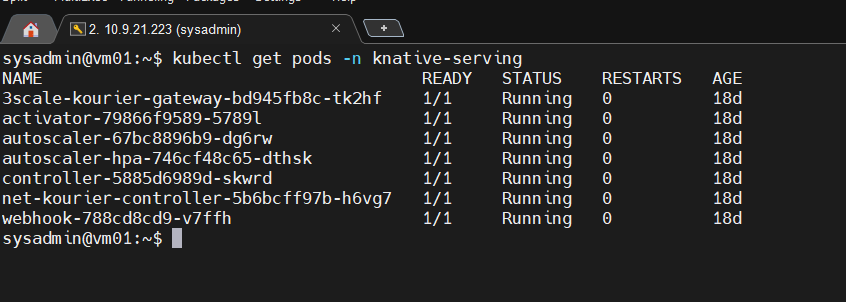
\includegraphics[width=0.92\textwidth]{image/capture_knative_pods.png}
    \caption{Composants de Knative Serving déployés sur le cluster}
    \label{fig:capture-knative-pods}
\end{figure}

\begin{itemize}
    \item \textbf{Services Knative créés par le backend dans un namespace tenant.}
\end{itemize}

La figure~\ref{fig:capture-ksvc} liste les ressources Service Knative du namespace \texttt{user-user}, créées par le backend via Fabric8, chacune avec une URL conforme à la convention \texttt{<app>.<namespace>.10.9.21.231.sslip.io} définie au Sprint 0. Deux services y apparaissent à l'état \texttt{READY: False} (motif \texttt{RevisionMissing}) : ces cas sont conservés dans la capture car ils illustrent que le suivi de statut remonte fidèlement les échecs de déploiement, la fonction attendue du \texttt{KnativeWatcher} développé au Sprint 5.

\begin{figure}[H]
 \centering
    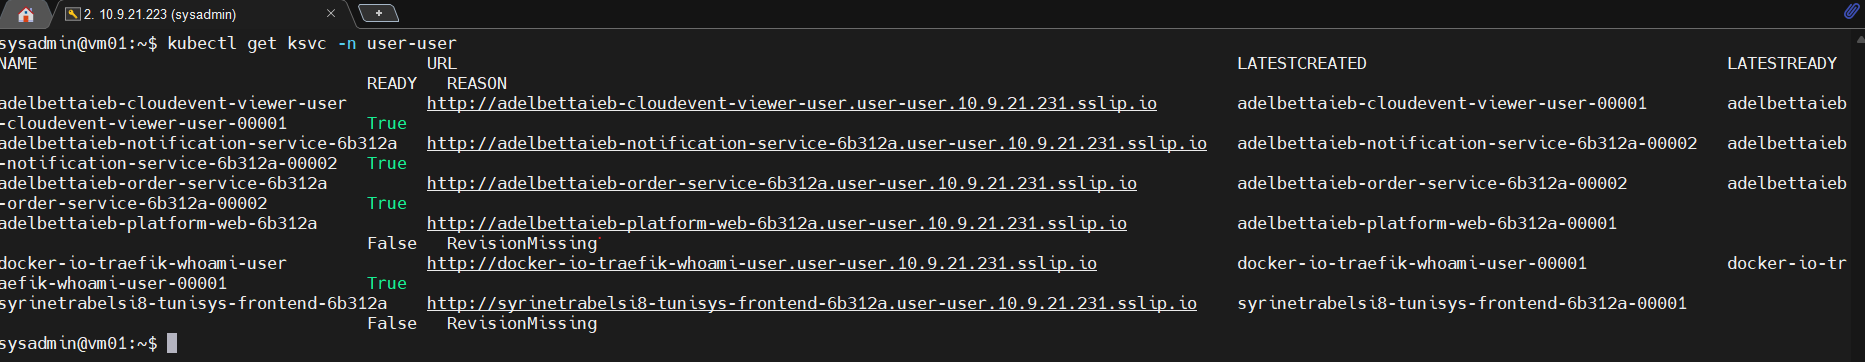
\includegraphics[width=\textwidth]{image/capture_ksvc_tenant.png}
    \caption{Services Knative d'un namespace tenant, créés par le backend}
    \label{fig:capture-ksvc}
\end{figure}

\subsubsection{Configuration et déploiement}

Le service Knative est créé avec les valeurs par défaut décrites en Conception (minScale 0, maxScale 10, port 8080, 100m CPU, 128Mi mémoire). Kourier, installé au Sprint 0, reçoit le trafic externe et le route vers la Revision active selon le nom d'hôte.

Deux limites sont à signaler : l'installation de Knative Serving elle-même n'est pas versionnée sous forme de manifestes, comme le socle du Sprint 0 ; et l'absence de client Java officiel a imposé le recours à l'API générique de Fabric8, plus verbeuse et moins sûre au niveau du typage — un choix assumé pour l'ensemble des ressources Kubernetes personnalisées du projet, par souci d'homogénéité.

À l'issue de ce sprint, le backend peut créer, par programmation, une application conteneurisée exécutée par Knative Serving, capable de monter en charge selon le trafic et de redescendre à zéro instance. Cette capacité sera exposée aux utilisateurs finaux à partir du Sprint 5.

\clearpage
\section{Sprint 2 : Mise en place de Kafka et Strimzi}

\subsection{Introduction}

La troisième brique répond à un besoin différent des deux précédentes : une plateforme serverless tire une bonne part de son intérêt de sa capacité à réagir à des événements plutôt qu'à de simples requêtes HTTP, ce qui suppose un bus de messages. Apache Kafka remplit ce rôle, déployé et administré par l'opérateur Strimzi plutôt qu'installé manuellement.

Ce sprint se limite à la gestion des topics par le backend : la publication et la consommation de messages relèvent de Knative Eventing (Sprint 3), et l'accès des clients à leurs propres topics n'arrivera qu'au Sprint 6, une fois le portail disponible.

\subsection{Objectifs du Sprint}

\begin{itemize}
    \item Déployer un cluster Apache Kafka opéré par l'opérateur Strimzi sur le cluster Kubernetes.
    \item Permettre au backend de créer, lister et supprimer des topics Kafka par programmation, via AdminClient.
\end{itemize}
\subsection{Sprint Backlog}
Le tableau~\ref{tab:sb-sprint2} présente le backlog détaillé du Sprint 2, obtenu en décomposant chaque User Story retenue en tâches techniques.

{
% Le tableau deborde volontairement de 1,5 cm dans chaque marge afin de laisser
% respirer les trois colonnes ; LTleft/LTright sont les parametres propres a
% longtable (adjustwidth n'a aucun effet sur cet environnement).
% Largeur totale : 18,8 cm, soit 1 cm de blanc conserve de chaque cote de la page.
\setlength{\LTleft}{-1.5cm}
\setlength{\LTright}{-1.5cm}
\setlength{\tabcolsep}{8pt}
\renewcommand{\arraystretch}{1.9}
\begin{longtable}{|p{6.6cm}|>{\raggedright\arraybackslash}p{8.1cm}|>{\centering\arraybackslash}p{2.3cm}|}
\hline
User Story & Tâches & Estimation \\
\hline
\endfirsthead
\hline
User Story & Tâches & Estimation \\
\hline
\endhead
\endfoot
\hline
\caption{Backlog du Sprint 2}
\label{tab:sb-sprint2}
\endlastfoot

\multirow{2}{6.6cm}{
\centering
En tant qu'ADMIN, je veux disposer d'un cluster Kafka opéré par Strimzi.
}
&
Provisionner l'opérateur Strimzi et un cluster Kafka, my-cluster, sur le cluster Kubernetes.
& 2 \\*
\cline{2-3}
&
Vérifier que le service de bootstrap my-cluster-kafka-bootstrap répond aux requêtes AdminClient.
& 1 \\
\hline

\multirow{3}{6.6cm}{
\centering
En tant que développeur backend, je veux pouvoir créer, lister et supprimer un topic Kafka par programmation.
}
&
Implémenter la création de topics via le client Kafka natif AdminClient.
& 2 \\*
\cline{2-3}
&
Implémenter le listing et la suppression de topics via AdminClient.
& 1 \\*
\hline
\cline{2-3}
&
Vérifier qu'un topic créé via AdminClient apparaît dans la liste des topics, et qu'un topic supprimé en disparaît.
& 1 \\
\hline
\end{longtable}
}

% \subsection{Sprint Backlog}

% Le tableau~\ref{tab:sb-sprint2} présente le backlog détaillé du Sprint 2, obtenu en décomposant chaque User Story retenue en tâches techniques.

% % \needspace garantit qu'il reste assez de place sur la page : sans cela une
% % coupure peut tomber au milieu d'un groupe \multirow, dont le contenu deborde
% % alors hors du cadre et laisse une cellule vide sur la page suivante.
% \needspace{0.75\textheight}
% {
% % Le tableau deborde volontairement de 1,5 cm dans chaque marge afin de laisser
% % respirer les trois colonnes ; LTleft/LTright sont les parametres propres a
% % longtable (adjustwidth n'a aucun effet sur cet environnement).
% % Largeur totale : 18,8 cm, soit 1 cm de blanc conserve de chaque cote de la page.
% \setlength{\LTleft}{-1.5cm}
% \setlength{\LTright}{-1.5cm}
% \setlength{\tabcolsep}{8pt}
% \renewcommand{\arraystretch}{1.9}
% \begin{longtable}{|p{6.6cm}|>{\raggedright\arraybackslash}p{8.1cm}|>{\centering\arraybackslash}p{2.3cm}|}
% \hline
% User Story & Tâches & Estimation \\
% \hline
% \endfirsthead
% \hline
% User Story & Tâches & Estimation \\
% \hline
% \endhead
% \endfoot
% \hline

% \caption{Backlog du Sprint 2}
% \label{tab:sb-sprint2}
% \endlastfoot

% \multirow{2}{6.6cm}{
% \centering
% En tant qu'ADMIN, je veux disposer d'un cluster Kafka opéré par Strimzi.
% }
% &
% Provisionner l'opérateur Strimzi et un cluster Kafka, my-cluster, sur le cluster Kubernetes.
% & — \\
% \cline{2-3}

% &
% Vérifier que le service de bootstrap my-cluster-kafka-bootstrap répond aux requêtes AdminClient.
% & — \\
% \hline

% \multirow{3}{6.6cm}{
% \centering
% En tant que développeur backend, je veux pouvoir créer, lister et supprimer un topic Kafka par programmation.
% }
% &
% Implémenter la création de topics via le client Kafka natif AdminClient.
% & — \\
% \cline{2-3}

% &
% Implémenter le listing et la suppression de topics via AdminClient.
% & — \\
% \cline{2-3}

% &
% Vérifier qu'un topic créé via AdminClient apparaît dans la liste des topics, et qu'un topic supprimé en disparaît.
% & — \\
% \hline

% \end{longtable}
% }

\subsection{Conception}

\subsubsection{Kafka : rôle dans la plateforme}

Knative Serving répond au besoin de faire tourner une application à la demande ; une plateforme serverless devient plus intéressante encore lorsque ce réveil peut être déclenché par un événement métier. C'est le rôle d'Apache Kafka \cite{KafkaDoc} : un bus d'événements où des composants communiquent de manière asynchrone, en publiant et consommant des messages plutôt qu'en s'appelant directement.

Un cluster Kafka repose sur des brokers, qui stockent les messages organisés en topics eux-mêmes subdivisés en partitions ; un producer publie, un consumer consomme. La figure~\ref{fig:kafka-concepts} résume ces rôles.

\begin{figure}[H]
\begin{adjustwidth}{-0.7cm}{-0.7cm}
\centering
\begin{tikzpicture}[
  x=1cm, y=1cm, every node/.style={font=\normalsize},
  act/.style={draw=figBleu, line width=1pt, rounded corners, minimum width=3.0cm,
              minimum height=1.3cm, align=center, fill=figBleuFond},
  part/.style={draw=figVert, line width=0.9pt, rounded corners, minimum width=1.6cm,
               minimum height=0.8cm, align=center, fill=white, font=\small},
  fl/.style={->, line width=1pt, figBleu}
]
\node[act] (prod) at (0,0)    {Producer};
\node[act] (cons) at (14.2,0) {Consumer};

% Cadres dessines d'abord, du plus englobant au plus interne, puis les partitions.
\draw[draw=figVert, line width=1.2pt, rounded corners, fill=figVertFond]
      (3.9,-1.8) rectangle (10.9,1.75);
\draw[draw=figVert, line width=1pt, rounded corners, fill=white]
      (4.35,-1.35) rectangle (10.45,0.65);

\node[part] (p0) at (5.4,-0.7) {partition 0};
\node[part] (p1) at (7.4,-0.7) {partition 1};
\node[part] (p2) at (9.4,-0.7) {partition 2};
\node[font=\small\bfseries, text=figVert] at (7.4,0.25) {Topic};
\node[font=\small\bfseries, text=figVert] at (7.4,1.35) {Broker Kafka};

\draw[fl] (prod.east) -- (3.9,0) node[midway, above, font=\small] {publie};
\draw[fl] (10.9,0) -- (cons.west) node[midway, above, font=\small] {consomme};
\end{tikzpicture}
\caption{Rôles fondamentaux d'un système Kafka}
\label{fig:kafka-concepts}
\end{adjustwidth}
\end{figure}

Dans la plateforme, Kafka sert de bus d'événements partagé entre applications clientes : l'une publie un événement sur un topic, une autre — potentiellement à zéro instance — est réveillée pour le traiter, via le mécanisme d'Eventing détaillé au Sprint 3.

\subsubsection{Strimzi : Kafka sur Kubernetes}

Kafka et Strimzi ne sont pas la même chose : Kafka est la plateforme de messagerie décrite ci-dessus ; Strimzi \cite{StrimziDoc} est l'opérateur Kubernetes qui l'exécute et l'administre directement sur l'infrastructure du projet.

\begin{figure}[H]
\begin{adjustwidth}{-1.0cm}{-1.0cm}
\centering
\begin{tikzpicture}[
  x=1cm, y=1cm, every node/.style={font=\normalsize},
  op/.style={draw=figOrange, line width=1pt, dashed, rounded corners, minimum width=5.6cm,
             minimum height=1.6cm, align=center, fill=figOrangeFond},
  br/.style={draw=figVert, line width=0.9pt, rounded corners, minimum width=2.4cm,
             minimum height=1.0cm, align=center, fill=white, font=\small},
  svc/.style={draw=figBleu, line width=1pt, rounded corners, minimum width=6.6cm,
              minimum height=1.5cm, align=center, fill=figBleuFond},
  note/.style={draw=black!45, dashed, line width=0.9pt, rounded corners, align=left,
               font=\small, fill=black!3}
]
\node[op] (strimzi) at (0,0)
     {Opérateur Strimzi\\[1pt]\small crée et administre le cluster Kafka};

\node[br] (b1) at (7.9,0)  {broker};
\node[br] (b2) at (10.6,0) {broker};
\node[br] (b3) at (13.3,0) {\dots};
\node[font=\small\bfseries, text=figVert] (klab) at (10.6,1.25) {Cluster Kafka \texttt{my-cluster}};

\node[svc] (boot) at (10.6,-3.4)
     {Service de bootstrap\\[1pt]\small point d'entrée interne généré par Strimzi};
\node[note] (nt) at (1.6,-3.4)
     {Écouteur interne en clair\\ni TLS ni SASL : c'est la voie\\empruntée par le backend};

\begin{scope}[on background layer]
  \node[draw=figVert, line width=1.2pt, rounded corners, inner sep=9pt, fill=figVertFond,
        fit=(b1)(b2)(b3)(klab)] (kafka) {};
\end{scope}

\draw[->, line width=1pt, figOrange, dashed] (strimzi.east) -- (kafka.west)
      node[midway, above, font=\scriptsize, fill=white, inner sep=1.5pt] {déploie et pilote};
\draw[->, line width=1pt, figVert] (kafka.south) -- (boot.north)
      node[midway, right, font=\scriptsize] {expose};

\begin{scope}[on background layer]
  \node[draw=black!50, dotted, line width=1pt, rounded corners, inner sep=15pt,
        fit=(strimzi)(kafka)(boot)(nt)] (ns) {};
\end{scope}
\node[font=\small\bfseries, text=black!65, anchor=south west]
      at ([yshift=3pt]ns.north west) {Cluster Kubernetes — namespace \texttt{kafka}};
\end{tikzpicture}
\caption{Relation entre Kubernetes, Strimzi et le cluster Kafka}
\label{fig:kafka-strimzi}
\end{adjustwidth}
\end{figure}

Le cluster Kafka de la plateforme (\texttt{my-cluster}) est opéré dans le namespace \texttt{kafka} et accessible en interne via le service de bootstrap standard généré par Strimzi. Ceci est confirmé par les variables d'environnement injectées aux applications clientes (Sprint 1). La connexion AdminClient du backend vers ce service ne configure ni TLS ni SASL. L'écouteur emprunté est donc en clair, ce qui reste acceptable tant que le trafic ne quitte pas le réseau interne du cluster.

\subsubsection{AdminClient, et non Fabric8}
\label{sec:kafka-adminclient}

Une distinction doit rester claire dans ce chapitre : Fabric8 pilote les ressources Kubernetes, Knative Serving et, au Sprint 3, Knative Eventing. Les topics Kafka, eux, ne passent pas par Fabric8 : bien que Strimzi expose une ressource personnalisée KafkaTopic, ce n'est pas le mécanisme retenu ici — créer un topic est une opération du protocole Kafka lui-même, gérée par la bibliothèque cliente AdminClient, indépendante de Kubernetes et ouverte directement vers les courtiers du cluster.

AdminClient permet de créer, lister et supprimer un topic ; son pilotage précis côté backend est présenté au chapitre qui lui est consacré (Release 1). Un nom du code peut prêter à confusion : la classe \texttt{KafkaTopic} du backend n'est pas la ressource Strimzi du même nom, mais une entité de persistance propre qui conserve en base les métadonnées de chaque topic client. La figure~\ref{fig:backend-kafka-adminclient} illustre la chaîne d'intégration réelle.

\begin{figure}[H]
\begin{adjustwidth}{-1.4cm}{-1.4cm}
\centering
\begin{tikzpicture}[
  x=1cm, y=1cm, every node/.style={font=\normalsize},
  acteur/.style={draw=black!65, line width=1.1pt, rounded corners, minimum width=4.4cm,
                 minimum height=1.3cm, align=center, fill=black!6},
  comp/.style={draw=figBleu, line width=1pt, rounded corners, minimum width=6.6cm,
               minimum height=1.4cm, align=center, fill=figBleuFond, font=\small},
  kfk/.style={draw=figOrange, line width=1pt, rounded corners, minimum width=6.6cm,
              minimum height=1.4cm, align=center, fill=figOrangeFond, font=\small},
  db/.style={draw=figVert, line width=1pt, rounded corners, minimum width=4.2cm,
             minimum height=1.4cm, align=center, fill=figVertFond, font=\small},
  hors/.style={draw=black!40, dotted, line width=1pt, rounded corners, align=left,
               font=\small, fill=black!3, text=black!60},
  zone/.style={rounded corners, inner sep=13pt, line width=1.1pt},
  num/.style={circle, draw, line width=0.8pt, fill=white, inner sep=2pt, font=\small\bfseries},
  et/.style={font=\small, align=left}
]

% ---------------- acteur ----------------
\node[acteur] (act) at (0,2.6) {CLIENT\_ADMIN\\[1pt]\footnotesize depuis le portail};

% ---------------- zone backend ----------------
\node[comp] (ctrl) at (0,-0.6)  {KafkaController / KafkaService\\\footnotesize vérifie les droits, résout le propriétaire};
\node[comp] (adm)  at (0,-3.1)  {AdminClient\\\footnotesize bibliothèque cliente du protocole Kafka};
\node[comp] (ent)  at (9.4,-0.6){entité \texttt{KafkaTopic} (JPA)\\\footnotesize métadonnées du topic};

\begin{scope}[on background layer]
  \node[zone, draw=figBleu, dashed, fill=figBleu!4, fit=(ctrl)(adm)(ent)] (zbk) {};
\end{scope}
\node[font=\small\bfseries, text=figBleu, anchor=south west, fill=white, inner sep=2pt] at ([yshift=3pt]zbk.north west)
     {Backend Spring Boot — namespace \texttt{platform}};

% ---------------- zone cluster kafka ----------------
\node[kfk] (boot) at (0,-7.9) {Service de bootstrap\\\footnotesize point d'entrée interne du cluster};
\node[kfk] (brok) at (0,-10.4) {Courtiers\\\footnotesize le topic est créé avec ses partitions};

\begin{scope}[on background layer]
  \node[zone, draw=figOrange, dashed, fill=figOrange!4, fit=(boot)(brok)] (zkf) {};
\end{scope}
\node[font=\small\bfseries, text=figOrange, anchor=south west, fill=white, inner sep=2pt] at ([yshift=3pt]zkf.north west)
     {Cluster Kafka \texttt{my-cluster} — namespace \texttt{kafka}};

% ---------------- base de donnees ----------------
\node[db] (pg) at (9.4,-3.1) {PostgreSQL};

% ---------------- fleches ----------------
\draw[->, line width=1pt, black!65] (act) -- (ctrl);
\draw[->, line width=1pt, figBleu]  (ctrl) -- (adm);
\draw[->, line width=1pt, figOrange](adm.south) -- (boot.north);
\draw[->, line width=1pt, figOrange](boot) -- (brok);
\draw[->, line width=1pt, figVert]  (ctrl.east) -- (ent.west);
\draw[->, line width=1pt, figVert]  (ent) -- (pg);

% ---------------- numeros et etapes ----------------
\node[num] at (0,1.45)  {1};
\node[num] at (0,-1.85) {2};
\node[num] at (0,-5.5)  {3};
\node[num] at (0,-9.15) {4};
\node[num] at (4.7,-0.6){5};
\node[num] at (9.4,-1.85){6};

\node[et, anchor=west] at (0.35,1.45)  {demande la création d'un topic};
\node[et, anchor=west] at (0.35,-1.85) {délègue au client Kafka};
\node[et, anchor=west, text=figOrange] at (0.35,-5.5)
     {ouvre une connexion vers les courtiers\\\footnotesize sans passer par l'API Kubernetes};
\node[et, anchor=west, text=figOrange] at (0.35,-9.15) {exécute \texttt{createTopics}};
\node[et, anchor=south] at (4.7,-0.35) {\footnotesize enregistre};
\node[et, anchor=west, text=figVert] at (9.75,-1.85) {\footnotesize persiste};

% ---------------- ce qui n'intervient pas ----------------
\node[hors] (nk) at (10.6,-9.15)
     {API Kubernetes\\
      n'intervient pas dans ce flux.\\
      Elle sert à Fabric8 pour Knative\\
      et l'Eventing. La ressource Strimzi\\
      \texttt{KafkaTopic} (CRD) n'est pas\\
      utilisée dans ce projet.};

\end{tikzpicture}
\caption{Chaîne d'intégration du backend au cluster Kafka via AdminClient}
\label{fig:backend-kafka-adminclient}
\end{adjustwidth}
\end{figure}

\subsection{Réalisation}

\subsubsection{Mise en œuvre}

Ce sprint livre le cluster Kafka opéré par Strimzi, ainsi que la capacité du backend à créer et gérer des topics par programmation ; son implémentation précise (persistance, contrôles d'accès) est présentée au chapitre consacré au backend (Release 1). Son exposition aux clients via une interface graphique ne sera livrée qu'au Sprint 6.

\begin{itemize}
    \item \textbf{Composants du cluster Kafka.}
\end{itemize}

La figure~\ref{fig:capture-kafka-pods} montre les pods du namespace \texttt{kafka} (opérateur \texttt{strimzi-cluster-operator}, courtier \texttt{my-cluster-kafka-0}, instance ZooKeeper et entity-operator), tous à l'état Running depuis dix-huit jours.

\begin{figure}[H]
 \centering
    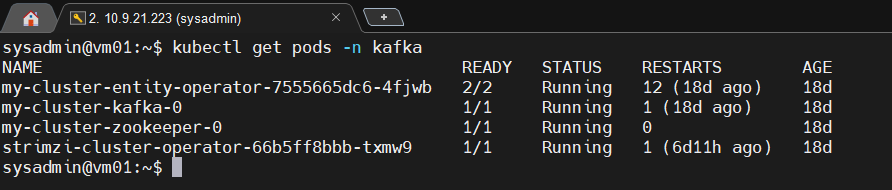
\includegraphics[width=0.92\textwidth]{image/capture_kafka_pods.png}
    \caption{Composants du cluster Kafka opéré par Strimzi}
    \label{fig:capture-kafka-pods}
\end{figure}

\begin{itemize}
    \item \textbf{Ressource Kafka gérée par l'opérateur.}
\end{itemize}

La figure~\ref{fig:capture-kafka-cluster} affiche la ressource personnalisée \texttt{Kafka} réconciliée par Strimzi, avec un courtier et une instance ZooKeeper désirés, à l'état \texttt{READY: True}, en mode ZooKeeper plutôt que KRaft.

\begin{figure}[H]
 \centering
    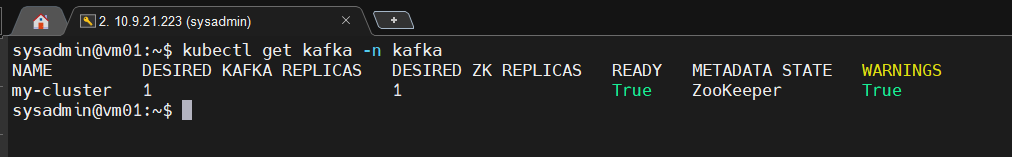
\includegraphics[width=0.92\textwidth]{image/capture_kafka_cluster.png}
    \caption{Ressource personnalisée \texttt{Kafka} réconciliée par l'opérateur Strimzi}
    \label{fig:capture-kafka-cluster}
\end{figure}

\begin{itemize}
    \item \textbf{Points d'accès réseau du cluster Kafka.}
\end{itemize}

La figure~\ref{fig:capture-kafka-svc} liste les services exposés dans le namespace \texttt{kafka}. Le backend contacte en interne le service \texttt{my-cluster-kafka-bootstrap} (\texttt{ClusterIP}) sur le port 9092.

\begin{figure}[H]
 \centering
    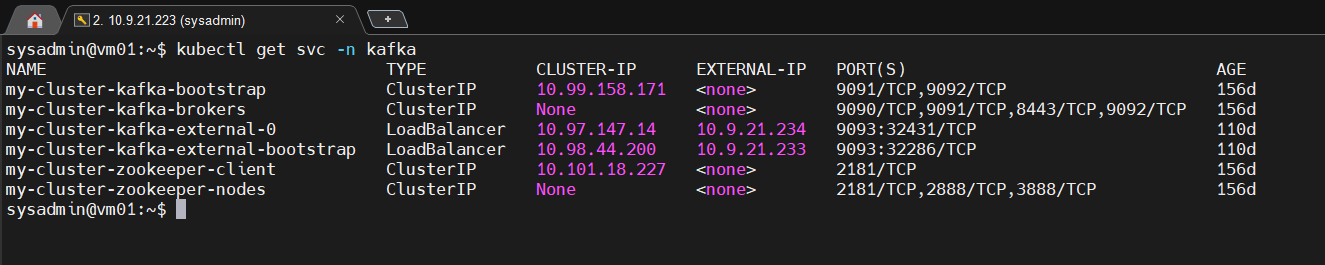
\includegraphics[width=\textwidth]{image/capture_kafka_svc.png}
    \caption{Services exposés par le cluster Kafka dans le namespace \texttt{kafka}}
    \label{fig:capture-kafka-svc}
\end{figure}

\subsubsection{Configuration et déploiement}

Le cluster Kafka \texttt{my-cluster} est provisionné dans le namespace \texttt{kafka} ; le backend s'y connecte via le service de bootstrap, sans authentification, sur le réseau interne. Comme les autres briques de ce socle, son installation n'est pas versionnée dans le dépôt, où seule la gestion applicative des topics via AdminClient figure.

L'inspection de la ressource \texttt{Kafka} précise le dimensionnement retenu : Strimzi 0.45.0, un courtier et une instance ZooKeeper, chacun adossé à un volume persistant de 1 Gio (\texttt{local-path}) — un dimensionnement d'environnement de développement, suffisant pour valider la chaîne fonctionnelle de cette release, qu'une exploitation réelle demanderait de renforcer (plusieurs courtiers, stockage répliqué).

Deux points d'accès \texttt{LoadBalancer} complètent le service de bootstrap interne, sur le port 9093, pour permettre la connexion d'outils de développement externes ; leur exposition constitue un risque assumé dans le périmètre de développement de ce projet.

Au terme de cette release, le cluster dispose des trois briques d'infrastructure fondamentales de la plateforme : orchestration Kubernetes isolée par tenant, exécution serverless via Knative Serving, et messagerie événementielle via Kafka et Strimzi. Le backend peut créer, lister et supprimer des topics Kafka par programmation ; cette capacité sera exposée aux clients via l'interface graphique à partir du Sprint 6.

\section{Conclusion}

La Release 0 a permis de construire, de manière incrémentale et validée à chaque étape, le socle cloud native de la plateforme : cluster Kubernetes isolé par tenant (Sprint 0), exécution serverless via Knative Serving (Sprint 1), bus d'événements Kafka opéré par Strimzi (Sprint 2). Cette approche progressive, conforme à la méthodologie Scrum retenue, a permis de valider chaque brique et d'en documenter honnêtement les mécanismes d'intégration réels, avant d'y adosser la logique métier présentée au chapitre suivant.
